% Emacs, this is -*-latex-*-
We now describe experiments and results focused on the key motivation of this work --- to facilitate 
analysis of a longitudinal study of individuals at risk for Alzheimer's disease (AD) where the statistical 
signal is weak (with small to medium sample sizes). We describe the dataset details followed by the analysis and then interpret our conclusions 
in the context of scientific results that have been published in the literature in aging and dementia.

%\subsection{Background}
\paragraph{Study background.} We analyzed data from a 
%unique  neuroimaging obtained through the Wisconsin Registry for Alzheimer's Prevention (WRAP), 
cohort of individuals who have been longitudinally tracked for at least three visits over multiple years, as part of an ongoing study (since 2001)
to understand the disease processes in the brain {\em before} an individual exhibits signs of 
cognitive decline due to Alzheimer's Disease (AD) \citep{sager2005middle}. The study, Wisconsin Registry for 
Alzheimer's Prevention (WRAP)  
is among the largest of its kind in existence, focused on ``preclinical'' AD, i.e., when the 
individuals are still cognitively healthy, offering a window into the early disease processes 
where treatments, drugs and interventions are likely to be most effective. 
%Many participants in this study have been longitudinally tracked for over ten years 
WRAP and its ancillary studies 
acquire neuroimaging data (MRI, PET with different tracers, diffusion MRI) and various clinical test scores, 
genetic and demographic data as well as clinical measures such as Cerebrospinal Fluid (CSF). Our analysis 
seeks to understand subtle group-wise differences in longitudinal patterns of dependencies between these measures at this early stage of the disease. 

\paragraph{Dataset.} The dataset consisted of 114 subjects with imaging data from at least two types of imaging modalities: Positron emission tomography and 
diffusion weighted Magnetic Resonance (MR) images. 
Positron emission tomography (PET) images were used to calculate, using well-validated pre-processing pipelines, 
the mean amyloid-plaque load (an important biomarker for AD) in 16 different anatomical regions of interest in the brain. 
Amyloid plaque is known to be an AD-related pathology and generally {\em precedes} onset of cognitive symptoms. 
Separately, diffusion tensor MR imaging (DTI) data were processed and used to calculate both Fractional Anisotropy (FA) and Mean Diffusivity (MD) in 48 distinct regions \citep{mori2008stereotaxic}. 
DTI images provide information about structural connectivity between gray matter regions in the brain. 
In addition to these $108$ ($48 \times 2 + 16$) image-derived features, 
we also included in the analysis the participant's scores on a battery of cognitive tests, known to be correlated with various neuropsychological functions \citep{lezak2004neuropsychological}. 
%One of the focus of of pre-clinical AD research is to identify biomarkers which may be reasonable indicators of developing pathology. 
%Identifying cognitive and neuroimaging measures that are significant differential trajectories could help in finding these biomarkers. 
%To detect group differences, grouping was performed using subject age, binned into three quantiles. 
Differences were evaluated on various groupings of the subjects which were, for the most part, 
based on known results in the literature.   
Specifically, gender, APOE (Apolipoprotein E) genotype and amyloid positivity (based on thresholding the amyloid plaque summaries) have 
all been evaluated as significant in
AD studies \citep{racine2014associations} but often such analyses involve a population covering a broader disease spectrum where 
the signal is much stronger. 
%Our cohort is still pre-sympotomatic.
%

\paragraph{Is analysis of second order statistics necessary?} In Figure \ref{fig:imagehists}, we present histograms detailing the distribution of two critical cognitive tests, stratified across various groups of scientific interest. Evaluating these distributions were the key motivation for our exploration into the methods described in this chapter. Small differences in means across groups {\em regardless of grouping selection (i.e., stratification variable)}, and the saturation that occurs at the ceiling of cognitive test scores and other preliminary experiments conducted by us suggest that standard analyses are not sensitive enough to identify subtle higher-order differences.
\begin{figure}
	\centering
	%\includegraphics[width=0.49\textwidth]{BNTHists.pdf}
	%\includegraphics[width=0.49\textwidth]{TTOTALHists.pdf}
	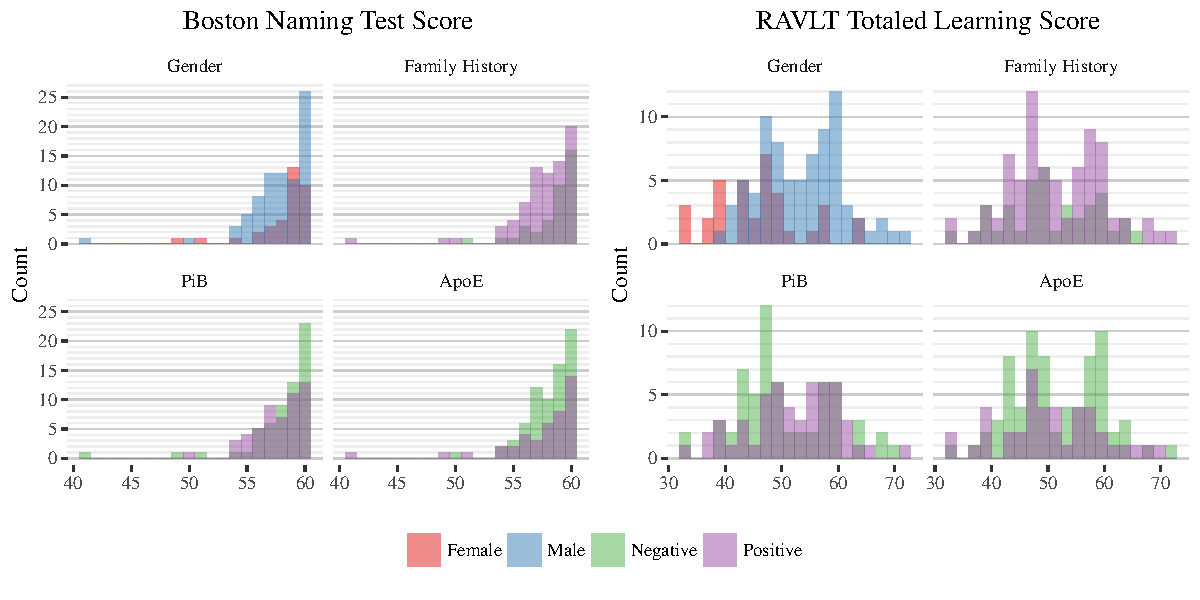
\includegraphics[width=\textwidth]{3_covtraj/figs/hists.pdf}
	\caption[Summary histograms of neuropsychological test scores for preclinical AD participants]{Histograms of the Boston Naming Test Scores and RAVLT Total Scores for all time points for the $114$ individual measurements across different group separations. The means for each test score is not significantly different across different stratification variable.}
	\label{fig:imagehists}
\end{figure}
\subsection{Results for Group difference analysis for individuals with imaging data}
We now describe, one by one, the components of the largest feature subset discovered for each stratification scheme 
and highlight the main scientific findings. In most cases, we provide a brief scientific interpretation of the results
for the interested reader. 
Additional details and results can be found in the appendix.
%, along with a longer description of our experimental setup and the covariate models learned for the significant groups.
%

\paragraph{A) Graph Scan Statistics on slope differences across gender.} 
The most significant (based on region-score) subset identified by the gender grouping was between the FA DTI measurement in the left cingulum gyrus 
as well as the scores on the Rey Auditory Verbal Learning Test (RAVLT). In recent AD research, gender has been identified as a factor in the progression 
of various pathology measures (e.g., incidence and prevalence of AD is higher in women \citep{fratiglioni1991prevalence,rimol2010sex}), and has contributed to a formal NIH notice (NOT-OD-15-102). However, we note that previous work in the field has \textit{not} identified gender-related 
differences when looking {\em only} at diffusion measures in the cingulum \citep{lin2014cingulum}. Our algorithm 
successfully identified longitudinal 
changes in {\em interaction} between these variables which supports the earlier results, and provides some evidence that as men and women age, 
their cognitive decline as measured by RAVLT manifests differently in relation to the cingulum gyrus.
%

\begin{table}
	\centering
	\begin{tabular}[t]{ll}
		\toprule
		\multicolumn{2}{c}{\textbf{Gender}}\\ \midrule \midrule
		
		Set 1     & RAVLT Total (1-5) \\ & FA Cingulum  L	\\
		\midrule
		Set 2 & FA Medial lemniscus L	\\ & FA Cingulum (hippocampus) L		\\
		& FA Post thalamic radiation L \\ \midrule
		Set 3    & FA Corticospinal tract R \\ & FA Superior O.F. fasciculus  R \\	\midrule\bottomrule
	\end{tabular}
	\hfill
	\begin{tabular}[t]{ll}
		\toprule
		\multicolumn{2}{c}{\textbf{Genotype: APOE4}}\\ \midrule \midrule
		Digit Span Backward Raw Score & Stroop Color-word Score \\ 
		PiB Cingulum Post L &    PiB Cingulum Post R         \\
		PiB Frontal Med Orb L & 		PiB Frontal Med Orb R \\ 
		PiB Precuneus L & PiB Precuneus R \\ 
		PiB SupraMarginal &  PiB Temporal Mid R \\ \midrule		 \bottomrule
	\end{tabular}
	\caption[Group differences identified across gender and genotype]{\label{tab:wrapIMG}Group difference across Gender (left) and Genotype APOE4 expression (right). Three disjoint sets of features were identified as coavarying significantly differently among gender, while one larger set was identified in the genotype stratification.}
\end{table}


\paragraph{B) Graph Scan Statistics on slope differences across genotype.} 
Next, we stratified the cohort
 based on the genotype known to be most closely linked with AD, i.e., the APOE (Apolipoprotein E) gene \citep{corder1993gene} --- 
we inherit one APOE allele from each parent; having one or two copies of the e4 allele increases a person's risk of getting AD 
whereas the rarer e2 allele is associated with a lower risk of AD. 
Using this stratification, we obtain a low-risk and an at-risk group of individuals. 
Here, we identified amyloid-load regions within the medial and lateral parietal lobes 
%with scores on the Controlled Oral Word Association fluency test \cite{abc}. The temporal gyrus is known to be stimulated when accessing word meaning while reading. Among the group without 
%this specific genotype risk allele, we 
and find that in the ``low-risk" group, the covariances between Digit Span and Stroop Color-Word scores 
(attention and concentration scores) and amyloid load moves from strongly negative towards $0$ as a function of age (Table \ref{tab:wrapIMG}). 
In the ``at-risk'' group 
(APOE4), however, we find that as a function of age, the features become more and more positively correlated. 
Existing studies have shown that the accumulation 
of amyloid is significantly different across APOE4 gene expression \citep{mormino2014amyloid}, and our results provide some evidence 
that the expression of the genotype may interact with cognitive scores as well, {\em even at this early stage of the disease}, 
when the individuals in our cohort are 
cognitively healthy. The sets of features showing a differential signal are presented in Table \ref{tab:wrapIMG}.
%has a real impact on the way in which one might solve language problems. (this sounds odd/needs elaboration)
%

\begin{table}
	\centering
	\begin{tabular}{lll}
		\toprule
		\multicolumn{3}{c}{\textbf{Amyloid Load (PiB Positivity)}}\\ \midrule \midrule
		%		    \multicolumn{3}{c}{Gender}}                   \\\
		Set 1 & PiB Angular L/R & PiB Cingulum Ant L/R \\
		& PiB Cingulum Post L/R & PiB Frontal Med Orb L/R \\
		& PiB Precuneus L/R & PiB Temporal Sup L/R \\
		& PiB Temporal Mid L/R & \textbf{PiB SupraMarginal L} \\
		\midrule
		Set 2     & FA Cerebral peduncle R   & FA Cerebral peduncle L	\\
		& MD Corticospinal tract R	& MD Corticospinal tract L		\\
		& Trail-Making Test Part A Score  & MD Cerebral peduncle R \\ 
		&PET Cingulum Post R  &  \\ \midrule\bottomrule
	\end{tabular}
	\caption{Group difference across Amyloid Load (PiB Positivity)}
	\label{tab:wrapPIB}
\end{table}

\paragraph{C) Graph Scan Statistics on slope differences across amyloid load positivity.} 
As briefly described above, amyloid load is an important biomarker for AD. For our analysis, amyloid (or PiB) positivity 
is calculated using the mean amyloid PiB measures across all brain regions using a PiB PET image scan of the participant. 
When we used this measure for stratification (threshold was set at $1.18$, following \cite{darst2017pathway}), 
our model identified fifteen of the sixteen PiB regions that were input to the model when the density of the oracle graph was set to be high. 
This result is as expected, but interestingly we find that controlling for the linear combination of the features (through centering), 
the residual error \textit{still} has significant signal with the PiB positivity measure, indicating that amyloid burden \textit{interactions} 
across brain regions plays a very important role in AD progression \citep{hardy2002amyloid,hardy1992alzheimer,tanzi2005twenty,jack2010brain}. When the sparsity of the oracle graph was increased, however, four neighboring regions, the left and right corticospinal tract and the left and right cerebral peduncle were identified on both PiB and DTI measures (supported by the literature \citep{douaud2011dti}), together with Part A of the Trail Making Test (see Table \ref{tab:wrapPIB}) which 
happens to be used in AD diagnosis \citep{albert2011diagnosis}. 
This suggests that changes in atrophy within these regions, as measured by DTI, co-occur with changes in amyloid burden. Additionally, because these regions are highly correlated with rough and fine motor ability \citep{naidich2009duvernoy}, it seems plausible that amyloid positivity will lead to higher `covariation' in the regions associated with 
a measure of fine motor speed, i.e., the Trail Making Test.

\subsection{Results for for Group difference analysis for individuals with Cognitive Testing data}

In addition to the dataset presented above, we apply our method to a much larger dataset consisting of approximately 1500 individuals with only cognitive testing data collected in a longitudinal manner. Each individual was administered these tests for between two and three time-points, yielding approximately $n = 4000$ samples for our model. For each assessment, a conference of experts applied a diagnostic label indicating normal cognition or mild cognitive impairment. Using this binary classification, we can stratify our population for group difference analysis.
We find that among many different significant subsets, the covariance trajectory among the scores on both parts of the Trail-Making Test and 
on all trials of the RAVLT test explain a significant group difference. These have previously been shown to be the {\em most sensitive tests} for 
early cognitive decline \citep{albert2001preclinical}. 
Table \ref{tab:wrapCC} displays the other tests identified by our algorithm, and additional experiments on this larger cohort 
can be found in the appendix. 
%

\begin{table}
	\centering
	\begin{tabular}{ll}
		\toprule
		\multicolumn{2}{c}{\textbf{Expert Consensus Diagnosis}}\\ \midrule \midrule
		WAIS-3 LNS Raw Score &
		Boston Naming Test Total Score \\
		RAVLT A2 Raw Score &
		RAVLT A3 Raw Score \\
		RAVLT A4 Raw Score &
		RAVLT A5 Raw Score \\
		RAVLT A6 Raw Score &
		RAVLT Delayed Recall Raw Score \\
		Trail-Making Test Part A &
		Trail-Making Test Part B \\
		Clock Drawing Test Score &
		CES Depression Scale Score \\
		\bottomrule
		\bottomrule
	\end{tabular}
	\caption[Localized results across expert clinical diagnosis]{Group difference localization across expert clinical diagnosis. With significantly more samples and a larger set of cognitive tests, those above were identified as significantly different across the expert consensus measure.}
	\label{tab:wrapCC}
\end{table}

\paragraph{Baseline.}
In various experiments on this dataset, when the MMGLM procedure is performed for the entire feature set in totality ({\em not} 
utilizing any of the proposed ideas based on scan statistics), 
and the null distribution derived using permutation testing, the procedure {\em yields no significance across \textit{any} 
scientifically interesting group stratifications}. 
This implies that the ability to search over different blocks of the covariance matrix is critical in identifying meaningful group differences 
in the trajectories, unavailable 
using alternate schemes. For instance, simpler strategies work well enough for datasets such as ADNI -- 
  which includes diseased subjects as well as controls -- 
  where the signal is stronger and even temporal modeling may be unnecessary.
  While the scientific results need to be interpreted with caution and reproducibility experiments on 
other similar datasets (both within the US and internationally) are in the planning phase, 
we believe that the ability to localize 
differences in these interaction patterns in a statistically rigorous manner is valuable and these findings can be investigated standalone, via 
more classical schemes (e.g., structural equation modeling). 


